\documentclass[]{article}
\usepackage{lmodern}
\usepackage{amssymb,amsmath}
\usepackage{ifxetex,ifluatex}
\usepackage{fixltx2e} % provides \textsubscript
\ifnum 0\ifxetex 1\fi\ifluatex 1\fi=0 % if pdftex
  \usepackage[T1]{fontenc}
  \usepackage[utf8]{inputenc}
\else % if luatex or xelatex
  \ifxetex
    \usepackage{mathspec}
  \else
    \usepackage{fontspec}
  \fi
  \defaultfontfeatures{Ligatures=TeX,Scale=MatchLowercase}
\fi
% use upquote if available, for straight quotes in verbatim environments
\IfFileExists{upquote.sty}{\usepackage{upquote}}{}
% use microtype if available
\IfFileExists{microtype.sty}{%
\usepackage[]{microtype}
\UseMicrotypeSet[protrusion]{basicmath} % disable protrusion for tt fonts
}{}
\PassOptionsToPackage{hyphens}{url} % url is loaded by hyperref
\usepackage[unicode=true]{hyperref}
\hypersetup{
            pdftitle={Project 1 - NSM724},
            pdfborder={0 0 0},
            breaklinks=true}
\urlstyle{same}  % don't use monospace font for urls
\usepackage[margin=1in]{geometry}
\usepackage{color}
\usepackage{fancyvrb}
\newcommand{\VerbBar}{|}
\newcommand{\VERB}{\Verb[commandchars=\\\{\}]}
\DefineVerbatimEnvironment{Highlighting}{Verbatim}{commandchars=\\\{\}}
% Add ',fontsize=\small' for more characters per line
\usepackage{framed}
\definecolor{shadecolor}{RGB}{248,248,248}
\newenvironment{Shaded}{\begin{snugshade}}{\end{snugshade}}
\newcommand{\KeywordTok}[1]{\textcolor[rgb]{0.13,0.29,0.53}{\textbf{#1}}}
\newcommand{\DataTypeTok}[1]{\textcolor[rgb]{0.13,0.29,0.53}{#1}}
\newcommand{\DecValTok}[1]{\textcolor[rgb]{0.00,0.00,0.81}{#1}}
\newcommand{\BaseNTok}[1]{\textcolor[rgb]{0.00,0.00,0.81}{#1}}
\newcommand{\FloatTok}[1]{\textcolor[rgb]{0.00,0.00,0.81}{#1}}
\newcommand{\ConstantTok}[1]{\textcolor[rgb]{0.00,0.00,0.00}{#1}}
\newcommand{\CharTok}[1]{\textcolor[rgb]{0.31,0.60,0.02}{#1}}
\newcommand{\SpecialCharTok}[1]{\textcolor[rgb]{0.00,0.00,0.00}{#1}}
\newcommand{\StringTok}[1]{\textcolor[rgb]{0.31,0.60,0.02}{#1}}
\newcommand{\VerbatimStringTok}[1]{\textcolor[rgb]{0.31,0.60,0.02}{#1}}
\newcommand{\SpecialStringTok}[1]{\textcolor[rgb]{0.31,0.60,0.02}{#1}}
\newcommand{\ImportTok}[1]{#1}
\newcommand{\CommentTok}[1]{\textcolor[rgb]{0.56,0.35,0.01}{\textit{#1}}}
\newcommand{\DocumentationTok}[1]{\textcolor[rgb]{0.56,0.35,0.01}{\textbf{\textit{#1}}}}
\newcommand{\AnnotationTok}[1]{\textcolor[rgb]{0.56,0.35,0.01}{\textbf{\textit{#1}}}}
\newcommand{\CommentVarTok}[1]{\textcolor[rgb]{0.56,0.35,0.01}{\textbf{\textit{#1}}}}
\newcommand{\OtherTok}[1]{\textcolor[rgb]{0.56,0.35,0.01}{#1}}
\newcommand{\FunctionTok}[1]{\textcolor[rgb]{0.00,0.00,0.00}{#1}}
\newcommand{\VariableTok}[1]{\textcolor[rgb]{0.00,0.00,0.00}{#1}}
\newcommand{\ControlFlowTok}[1]{\textcolor[rgb]{0.13,0.29,0.53}{\textbf{#1}}}
\newcommand{\OperatorTok}[1]{\textcolor[rgb]{0.81,0.36,0.00}{\textbf{#1}}}
\newcommand{\BuiltInTok}[1]{#1}
\newcommand{\ExtensionTok}[1]{#1}
\newcommand{\PreprocessorTok}[1]{\textcolor[rgb]{0.56,0.35,0.01}{\textit{#1}}}
\newcommand{\AttributeTok}[1]{\textcolor[rgb]{0.77,0.63,0.00}{#1}}
\newcommand{\RegionMarkerTok}[1]{#1}
\newcommand{\InformationTok}[1]{\textcolor[rgb]{0.56,0.35,0.01}{\textbf{\textit{#1}}}}
\newcommand{\WarningTok}[1]{\textcolor[rgb]{0.56,0.35,0.01}{\textbf{\textit{#1}}}}
\newcommand{\AlertTok}[1]{\textcolor[rgb]{0.94,0.16,0.16}{#1}}
\newcommand{\ErrorTok}[1]{\textcolor[rgb]{0.64,0.00,0.00}{\textbf{#1}}}
\newcommand{\NormalTok}[1]{#1}
\usepackage{graphicx,grffile}
\makeatletter
\def\maxwidth{\ifdim\Gin@nat@width>\linewidth\linewidth\else\Gin@nat@width\fi}
\def\maxheight{\ifdim\Gin@nat@height>\textheight\textheight\else\Gin@nat@height\fi}
\makeatother
% Scale images if necessary, so that they will not overflow the page
% margins by default, and it is still possible to overwrite the defaults
% using explicit options in \includegraphics[width, height, ...]{}
\setkeys{Gin}{width=\maxwidth,height=\maxheight,keepaspectratio}
\IfFileExists{parskip.sty}{%
\usepackage{parskip}
}{% else
\setlength{\parindent}{0pt}
\setlength{\parskip}{6pt plus 2pt minus 1pt}
}
\setlength{\emergencystretch}{3em}  % prevent overfull lines
\providecommand{\tightlist}{%
  \setlength{\itemsep}{0pt}\setlength{\parskip}{0pt}}
\setcounter{secnumdepth}{0}
% Redefines (sub)paragraphs to behave more like sections
\ifx\paragraph\undefined\else
\let\oldparagraph\paragraph
\renewcommand{\paragraph}[1]{\oldparagraph{#1}\mbox{}}
\fi
\ifx\subparagraph\undefined\else
\let\oldsubparagraph\subparagraph
\renewcommand{\subparagraph}[1]{\oldsubparagraph{#1}\mbox{}}
\fi

% set default figure placement to htbp
\makeatletter
\def\fps@figure{htbp}
\makeatother

\usepackage{etoolbox}
\makeatletter
\providecommand{\subtitle}[1]{% add subtitle to \maketitle
  \apptocmd{\@title}{\par {\large #1 \par}}{}{}
}
\makeatother
% https://github.com/rstudio/rmarkdown/issues/337
\let\rmarkdownfootnote\footnote%
\def\footnote{\protect\rmarkdownfootnote}

% https://github.com/rstudio/rmarkdown/pull/252
\usepackage{titling}
\setlength{\droptitle}{-2em}

\pretitle{\vspace{\droptitle}\centering\huge}
\posttitle{\par}

\preauthor{\centering\large\emph}
\postauthor{\par}

\predate{\centering\large\emph}
\postdate{\par}

\title{Project 1 - NSM724}
\date{}

\begin{document}
\maketitle

\subsection{Introduction}\label{introduction}

This project focuses on two datasets named ``drinks'' and ``healthgdp''.
``drinks'' is a dataset from fivethirtyeight which gives liters and
servings of alcohol consumption per capita in every country.
``healthgdp'' contains data released by the World Health Organization
which gives info about the percentage of the yearly GDP that is spent on
healthcare in every country. It also assigns each country to a region. I
will be joining these datasets and analyzing the data in the hopes of
seeing the habits of alcohol consumption in each region. I am also
interested to see if there will be an association between percentage of
GDP spent on healthcare and total alcohol consumption.

\begin{Shaded}
\begin{Highlighting}[]
\KeywordTok{library}\NormalTok{(tidyverse)}
\end{Highlighting}
\end{Shaded}

\begin{verbatim}
## ── Attaching packages ───────────────────────────────────────────── tidyverse 1.3.0 ──
\end{verbatim}

\begin{verbatim}
## ✓ ggplot2 3.2.1     ✓ purrr   0.3.3
## ✓ tibble  2.1.3     ✓ dplyr   0.8.3
## ✓ tidyr   1.0.0     ✓ stringr 1.4.0
## ✓ readr   1.3.1     ✓ forcats 0.4.0
\end{verbatim}

\begin{verbatim}
## ── Conflicts ──────────────────────────────────────────────── tidyverse_conflicts() ──
## x dplyr::filter() masks stats::filter()
## x dplyr::lag()    masks stats::lag()
\end{verbatim}

\begin{Shaded}
\begin{Highlighting}[]
\KeywordTok{library}\NormalTok{(fivethirtyeight)}

\KeywordTok{library}\NormalTok{(readxl)}
\NormalTok{healthgdp <-}\StringTok{ }\KeywordTok{read_excel}\NormalTok{(}\StringTok{"~/Desktop/gdp data2.xlsx"}\NormalTok{)}
\end{Highlighting}
\end{Shaded}

Here is a preview of the datasets.

\begin{Shaded}
\begin{Highlighting}[]
\KeywordTok{head}\NormalTok{(drinks)}
\end{Highlighting}
\end{Shaded}

\begin{verbatim}
## # A tibble: 6 x 5
##   country      beer_servings spirit_servings wine_servings total_litres_of_pure…
##   <chr>                <int>           <int>         <int>                 <dbl>
## 1 Afghanistan              0               0             0                   0  
## 2 Albania                 89             132            54                   4.9
## 3 Algeria                 25               0            14                   0.7
## 4 Andorra                245             138           312                  12.4
## 5 Angola                 217              57            45                   5.9
## 6 Antigua & B…           102             128            45                   4.9
\end{verbatim}

\begin{Shaded}
\begin{Highlighting}[]
\KeywordTok{head}\NormalTok{(healthgdp)}
\end{Highlighting}
\end{Shaded}

\begin{verbatim}
## # A tibble: 6 x 3
##   country     GDP_pct region                   
##   <chr>         <dbl> <chr>                    
## 1 Aruba         NA    Latin America & Caribbean
## 2 Afghanistan    8.57 South Asia               
## 3 Angola         2.74 Sub-Saharan Africa       
## 4 Albania        5.01 Europe & Central Asia    
## 5 Andorra        9.45 Europe & Central Asia    
## 6 Arab World     3.99 <NA>
\end{verbatim}

\subsection{Tidying}\label{tidying}

The ``drinks'' dataset is not tidy so the pivot\_longer function will be
used on it. The servings columns are actually values of a variable -
type of alcohol. A new column called ``type'' will be created in order
to indicate this. The original values of those columns will be placed in
a column called ``servings''. Before doing all of this, the original
column titles will be changed in order to be more clear.

\begin{Shaded}
\begin{Highlighting}[]
\NormalTok{drinks<-drinks}\OperatorTok\KeywordTok{rename}\NormalTok{(}
    \DataTypeTok{beer =}\NormalTok{ beer_servings,}
    \DataTypeTok{wine =}\NormalTok{ wine_servings,}
    \DataTypeTok{spirit =}\NormalTok{ spirit_servings}
\NormalTok{    )}
\NormalTok{drinks<-}\KeywordTok{pivot_longer}\NormalTok{(drinks,}\KeywordTok{c}\NormalTok{(}\StringTok{"beer"}\NormalTok{,}\StringTok{"spirit"}\NormalTok{,}\StringTok{"wine"}\NormalTok{),}\DataTypeTok{names_to =} \StringTok{"type"}\NormalTok{,}\DataTypeTok{values_to =} \StringTok{"servings"}\NormalTok{)}
\KeywordTok{head}\NormalTok{(drinks)}
\end{Highlighting}
\end{Shaded}

\begin{verbatim}
## # A tibble: 6 x 4
##   country     total_litres_of_pure_alcohol type   servings
##   <chr>                              <dbl> <chr>     <int>
## 1 Afghanistan                          0   beer          0
## 2 Afghanistan                          0   spirit        0
## 3 Afghanistan                          0   wine          0
## 4 Albania                              4.9 beer         89
## 5 Albania                              4.9 spirit      132
## 6 Albania                              4.9 wine         54
\end{verbatim}

\subsection{Joining}\label{joining}

Now that both datasets are tidy, they can be joined. I am using a left
join with ``drinks'' on the left because the ``healthgdp'' dataset
contains several ``country'' values that are not actually countries, but
regions or economic groupings. Other than that, no other rows should be
dropped. There are some countries in the ``drinks'' dataset that do not
appear in the ``healthgdp'' dataset so there are a handful of NA cases.
The full dataset will be named ``project1''.

\begin{Shaded}
\begin{Highlighting}[]
\NormalTok{project1<-}\KeywordTok{left_join}\NormalTok{(drinks,healthgdp)}
\end{Highlighting}
\end{Shaded}

\begin{verbatim}
## Joining, by = "country"
\end{verbatim}

\begin{Shaded}
\begin{Highlighting}[]
\KeywordTok{head}\NormalTok{(project1)}
\end{Highlighting}
\end{Shaded}

\begin{verbatim}
## # A tibble: 6 x 6
##   country    total_litres_of_pure_alc… type   servings GDP_pct region           
##   <chr>                          <dbl> <chr>     <int>   <dbl> <chr>            
## 1 Afghanist…                       0   beer          0    8.57 South Asia       
## 2 Afghanist…                       0   spirit        0    8.57 South Asia       
## 3 Afghanist…                       0   wine          0    8.57 South Asia       
## 4 Albania                          4.9 beer         89    5.01 Europe & Central…
## 5 Albania                          4.9 spirit      132    5.01 Europe & Central…
## 6 Albania                          4.9 wine         54    5.01 Europe & Central…
\end{verbatim}

\subsection{Wrangling}\label{wrangling}

It's time to see some summary statistics. For the sake of simplicity,
any NA rows will be removed from here on out. I wanted the full dataset
to contain every country which is why I didn't do an inner join earlier.
Now that we are looking at statistics, however, it is necessary to
remove the NA rows.

\begin{Shaded}
\begin{Highlighting}[]
\NormalTok{project1<-project1}\OperatorTok\NormalTok{na.omit}
\NormalTok{project1}\OperatorTok\KeywordTok{group_by}\NormalTok{(region)}\OperatorTok\KeywordTok{summarise}\NormalTok{(}\DataTypeTok{mean_GDP=}\KeywordTok{mean}\NormalTok{(GDP_pct),}\DataTypeTok{sd_GDP=}\KeywordTok{sd}\NormalTok{(GDP_pct))}\OperatorTok\KeywordTok{arrange}\NormalTok{(mean_GDP)}
\end{Highlighting}
\end{Shaded}

\begin{verbatim}
## # A tibble: 7 x 3
##   region                     mean_GDP sd_GDP
##   <chr>                         <dbl>  <dbl>
## 1 South Asia                     4.72   2.37
## 2 Middle East & North Africa     4.86   2.02
## 3 Sub-Saharan Africa             5.86   2.53
## 4 East Asia & Pacific            6.44   4.36
## 5 Latin America & Caribbean      6.73   1.52
## 6 Europe & Central Asia          7.70   2.30
## 7 North America                 10.6    0
\end{verbatim}

\begin{Shaded}
\begin{Highlighting}[]
\NormalTok{project1}\OperatorTok\KeywordTok{summarise}\NormalTok{(}\DataTypeTok{max_GDP=}\KeywordTok{max}\NormalTok{(GDP_pct),}\DataTypeTok{min_GDP=}\KeywordTok{min}\NormalTok{(GDP_pct),}\DataTypeTok{max_liters=}\KeywordTok{max}\NormalTok{(total_litres_of_pure_alcohol),}\DataTypeTok{min_liters=}\KeywordTok{min}\NormalTok{(total_litres_of_pure_alcohol),}\DataTypeTok{max_servings=}\KeywordTok{max}\NormalTok{(servings),}\DataTypeTok{min_servings=}\KeywordTok{min}\NormalTok{(servings))}
\end{Highlighting}
\end{Shaded}

\begin{verbatim}
## # A tibble: 1 x 6
##   max_GDP min_GDP max_liters min_liters max_servings min_servings
##     <dbl>   <dbl>      <dbl>      <dbl>        <int>        <int>
## 1    19.3    1.43       14.4          0          438            0
\end{verbatim}

I've calculated the mean percentage of GDP spent on healthcare in each
region. North America appears to be spending the most by far. I've also
found the maximum and minimum of each numeric variable in order to get
an idea of the range of this data.

Next, I'm going to see the mean and standard deviation of servings and
liters of alcohol consumed in each region. For servings I'm also
grouping by type of alcohol. I'm arranging from highest to lowest
consumption so I can get an idea of how much alcohol each region
consumes.

\begin{Shaded}
\begin{Highlighting}[]
\NormalTok{project1}\OperatorTok\KeywordTok{group_by}\NormalTok{(region,type)}\OperatorTok\KeywordTok{summarise}\NormalTok{(}\DataTypeTok{mean_servings=}\KeywordTok{mean}\NormalTok{(servings),}\DataTypeTok{sd_servings=}\KeywordTok{sd}\NormalTok{(servings))}\OperatorTok\KeywordTok{arrange}\NormalTok{(}\KeywordTok{desc}\NormalTok{(mean_servings))}
\end{Highlighting}
\end{Shaded}

\begin{verbatim}
## # A tibble: 21 x 4
## # Groups:   region [7]
##    region                    type   mean_servings sd_servings
##    <chr>                     <chr>          <dbl>       <dbl>
##  1 North America             beer           240          NA  
##  2 Europe & Central Asia     beer           188.        106. 
##  3 Latin America & Caribbean spirit         145.        102. 
##  4 Latin America & Caribbean beer           144.         71.7
##  5 Europe & Central Asia     wine           132.        103. 
##  6 Europe & Central Asia     spirit         131.         82.5
##  7 North America             spirit         122          NA  
##  8 North America             wine           100          NA  
##  9 East Asia & Pacific       beer            73.6        78.1
## 10 Sub-Saharan Africa        beer            70.4        88.4
## # … with 11 more rows
\end{verbatim}

\begin{Shaded}
\begin{Highlighting}[]
\NormalTok{project1}\OperatorTok\KeywordTok{group_by}\NormalTok{(region)}\OperatorTok
\StringTok{  }\KeywordTok{summarise}\NormalTok{(}\DataTypeTok{mean_liters=}\KeywordTok{mean}\NormalTok{(total_litres_of_pure_alcohol),}\DataTypeTok{sd_liters=}\KeywordTok{sd}\NormalTok{(total_litres_of_pure_alcohol))}\OperatorTok
\StringTok{  }\KeywordTok{arrange}\NormalTok{(}\KeywordTok{desc}\NormalTok{(mean_liters))}
\end{Highlighting}
\end{Shaded}

\begin{verbatim}
## # A tibble: 7 x 3
##   region                     mean_liters sd_liters
##   <chr>                            <dbl>     <dbl>
## 1 Europe & Central Asia            8.28      3.74 
## 2 North America                    8.2       0    
## 3 Latin America & Caribbean        5.83      2.24 
## 4 Sub-Saharan Africa               3.42      2.75 
## 5 East Asia & Pacific              2.92      2.98 
## 6 Middle East & North Africa       1.36      1.61 
## 7 South Asia                       0.625     0.939
\end{verbatim}

I wonder if there is a correlation between healthcare spending and
alcohol consumption. For the next part, I am going to create a new
column that represents total servings of alcohol per person and then see
if there is a correlation between that and healthcare spending. I'll do
the same with total liters of alcohol. Finally, I'll see how strong the
correlation between liters of alcohol consumed and servings of alcohol
consumed is.

\begin{Shaded}
\begin{Highlighting}[]
\NormalTok{project1<-project1}\OperatorTok\KeywordTok{group_by}\NormalTok{(country)}\OperatorTok\KeywordTok{mutate}\NormalTok{(}\DataTypeTok{total_servings=}\KeywordTok{sum}\NormalTok{(servings))}\OperatorTok\KeywordTok{ungroup}\NormalTok{(country)}
\KeywordTok{head}\NormalTok{(project1)}
\end{Highlighting}
\end{Shaded}

\begin{verbatim}
## # A tibble: 6 x 7
##   country   total_litres_of_pu… type  servings GDP_pct region     total_servings
##   <chr>                   <dbl> <chr>    <int>   <dbl> <chr>               <int>
## 1 Afghanis…                 0   beer         0    8.57 South Asia              0
## 2 Afghanis…                 0   spir…        0    8.57 South Asia              0
## 3 Afghanis…                 0   wine         0    8.57 South Asia              0
## 4 Albania                   4.9 beer        89    5.01 Europe & …            275
## 5 Albania                   4.9 spir…      132    5.01 Europe & …            275
## 6 Albania                   4.9 wine        54    5.01 Europe & …            275
\end{verbatim}

\begin{Shaded}
\begin{Highlighting}[]
\NormalTok{project1}\OperatorTok\KeywordTok{select}\NormalTok{(total_litres_of_pure_alcohol,GDP_pct)}\OperatorTok\NormalTok{cor}
\end{Highlighting}
\end{Shaded}

\begin{verbatim}
##                              total_litres_of_pure_alcohol   GDP_pct
## total_litres_of_pure_alcohol                    1.0000000 0.3977563
## GDP_pct                                         0.3977563 1.0000000
\end{verbatim}

\begin{Shaded}
\begin{Highlighting}[]
\NormalTok{project1}\OperatorTok\KeywordTok{select}\NormalTok{(total_servings,GDP_pct)}\OperatorTok\NormalTok{cor}
\end{Highlighting}
\end{Shaded}

\begin{verbatim}
##                total_servings   GDP_pct
## total_servings      1.0000000 0.3575527
## GDP_pct             0.3575527 1.0000000
\end{verbatim}

\begin{Shaded}
\begin{Highlighting}[]
\NormalTok{project1}\OperatorTok\KeywordTok{select}\NormalTok{(total_litres_of_pure_alcohol,total_servings)}\OperatorTok\NormalTok{cor}
\end{Highlighting}
\end{Shaded}

\begin{verbatim}
##                              total_litres_of_pure_alcohol total_servings
## total_litres_of_pure_alcohol                    1.0000000      0.9395312
## total_servings                                  0.9395312      1.0000000
\end{verbatim}

There is a small correlation between GDP and liters/servings of alcohol.
There is a strong correlation between liters and servings of alcohol
consumed which makes sense.

Going back to the previous summary stats, I am wondering why the percent
GDP spent on healthcare is so high in North America and why there are
NAs for this row. I'm going to look at the individual healthcare
spending for all North American countries to get a better idea.

\begin{Shaded}
\begin{Highlighting}[]
\NormalTok{project1}\OperatorTok\KeywordTok{filter}\NormalTok{(region}\OperatorTok{==}\StringTok{"North America"}\NormalTok{)}\OperatorTok\KeywordTok{select}\NormalTok{(country,GDP_pct)}
\end{Highlighting}
\end{Shaded}

\begin{verbatim}
## # A tibble: 3 x 2
##   country GDP_pct
##   <chr>     <dbl>
## 1 Canada     10.6
## 2 Canada     10.6
## 3 Canada     10.6
\end{verbatim}

Uh oh, there is only one country in the North America region! After
looking through the data, I have found that USA is not in the drinks
dataset so it was dropped during the left join. Mexico is classified as
Latin America so Canada is the only country representing North America.
This has prompted me to see how many countries are in each region to
make sure this isn't happening to other regions I am studying

\begin{Shaded}
\begin{Highlighting}[]
\NormalTok{project1}\OperatorTok\KeywordTok{group_by}\NormalTok{(region)}\OperatorTok\KeywordTok{summarise}\NormalTok{(}\DataTypeTok{country_count=}\KeywordTok{n_distinct}\NormalTok{(country))}
\end{Highlighting}
\end{Shaded}

\begin{verbatim}
## # A tibble: 7 x 2
##   region                     country_count
##   <chr>                              <int>
## 1 East Asia & Pacific                   25
## 2 Europe & Central Asia                 46
## 3 Latin America & Caribbean             27
## 4 Middle East & North Africa            16
## 5 North America                          1
## 6 South Asia                             8
## 7 Sub-Saharan Africa                    41
\end{verbatim}

Luckily, all of the other regions have more than one country.

\subsection{Visualization}\label{visualization}

Now that I have done some summary statistics and am more familiar with
the layout of the data, I'm going to make a couple plots.

\begin{Shaded}
\begin{Highlighting}[]
\NormalTok{project1}\OperatorTok\KeywordTok{ggplot}\NormalTok{(}\KeywordTok{aes}\NormalTok{(total_litres_of_pure_alcohol,total_servings))}\OperatorTok{+}
\StringTok{  }\KeywordTok{xlab}\NormalTok{(}\StringTok{"Total Liters Consumed"}\NormalTok{)}\OperatorTok{+}\KeywordTok{ylab}\NormalTok{(}\StringTok{"Total Servings Consumed"}\NormalTok{)}\OperatorTok{+}
\StringTok{  }\KeywordTok{ggtitle}\NormalTok{(}\StringTok{"Total Alcohol Consumption by Region"}\NormalTok{)}\OperatorTok{+}\KeywordTok{labs}\NormalTok{(}\DataTypeTok{color=}\StringTok{"Region"}\NormalTok{)}\OperatorTok{+}
\StringTok{  }\KeywordTok{theme}\NormalTok{(}\DataTypeTok{legend.position =} \StringTok{"left"}\NormalTok{)}\OperatorTok{+}
\StringTok{  }\KeywordTok{geom_point}\NormalTok{(}\KeywordTok{aes}\NormalTok{(}\DataTypeTok{color=}\NormalTok{region))}\OperatorTok{+}
\StringTok{  }\KeywordTok{scale_y_continuous}\NormalTok{(}\DataTypeTok{breaks=}\KeywordTok{c}\NormalTok{(}\DecValTok{0}\NormalTok{,}\DecValTok{100}\NormalTok{,}\DecValTok{200}\NormalTok{,}\DecValTok{300}\NormalTok{,}\DecValTok{400}\NormalTok{,}\DecValTok{500}\NormalTok{,}\DecValTok{600}\NormalTok{,}\DecValTok{700}\NormalTok{))}\OperatorTok{+}\KeywordTok{scale_color_hue}\NormalTok{(}\DataTypeTok{c=}\DecValTok{150}\NormalTok{)}
\end{Highlighting}
\end{Shaded}

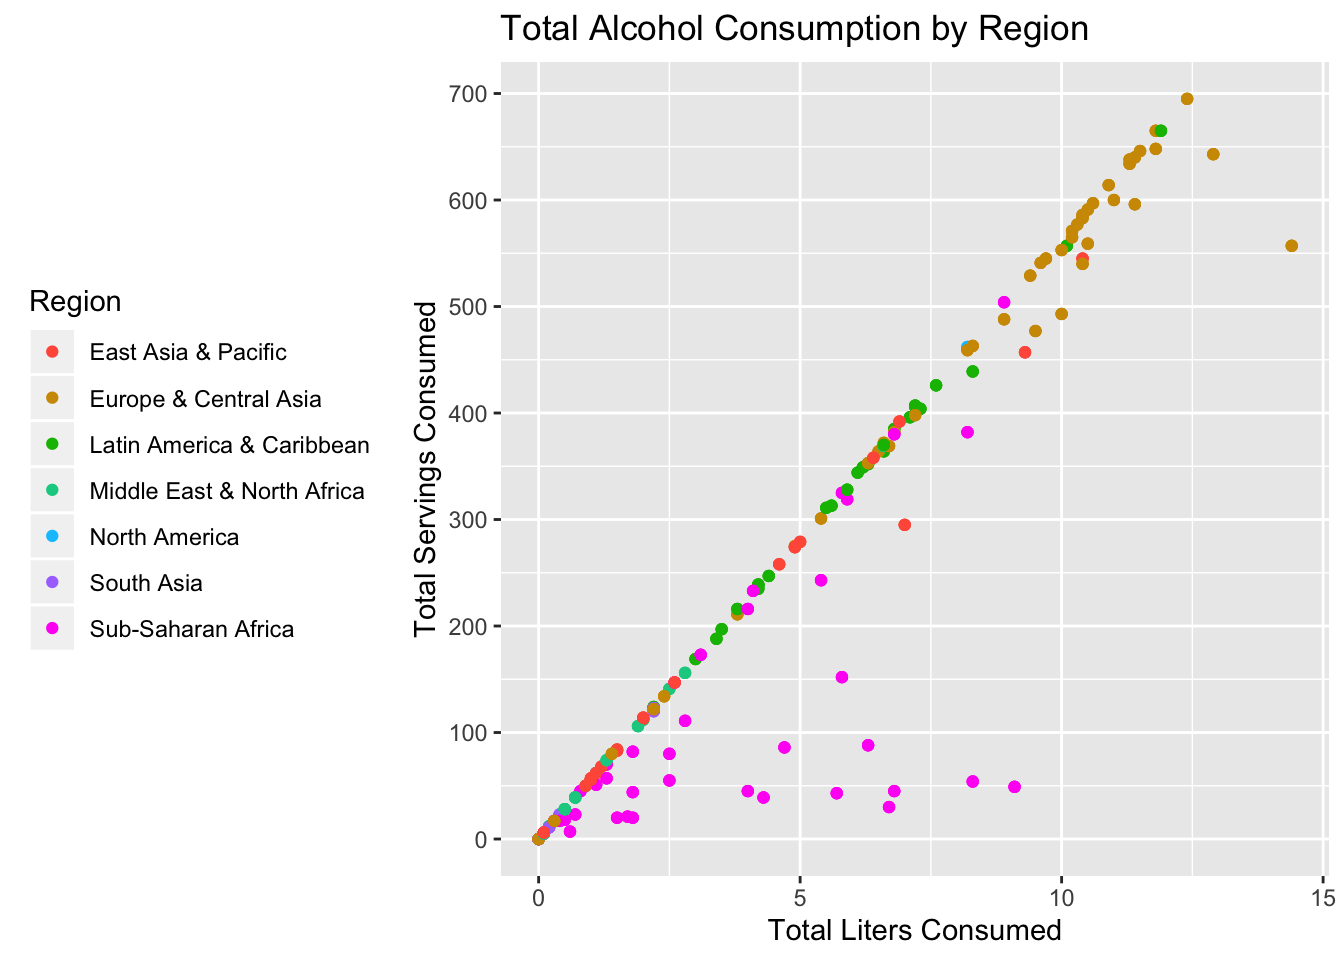
\includegraphics{project1_files/figure-latex/unnamed-chunk-10-1.pdf}

For the most part, there is a very strong correlation between total
liters of alcohol consumed and total servings consumed. By associating
each region with a color, we can see that the majority of countries that
do not follow this trend are in Sub-Saharan Africa. It seems that there
are a lot of European/Central Asian countries consuming the most
alcohol, while the Sub-Saharan African countries are consuming the
fewest servings.

\begin{Shaded}
\begin{Highlighting}[]
\NormalTok{project1}\OperatorTok\KeywordTok{ggplot}\NormalTok{(}\KeywordTok{aes}\NormalTok{(region,servings,}\DataTypeTok{fill=}\NormalTok{type))}\OperatorTok{+}
\StringTok{  }\KeywordTok{geom_bar}\NormalTok{(}\DataTypeTok{stat=}\StringTok{"summary"}\NormalTok{,}\DataTypeTok{fun.y=}\StringTok{"mean"}\NormalTok{,}\DataTypeTok{position =} \StringTok{"dodge"}\NormalTok{)}\OperatorTok{+}
\StringTok{  }\KeywordTok{theme}\NormalTok{(}\DataTypeTok{axis.text.x =} \KeywordTok{element_text}\NormalTok{(}\DataTypeTok{angle=}\DecValTok{45}\NormalTok{, }\DataTypeTok{hjust=}\DecValTok{1}\NormalTok{))}\OperatorTok{+}\KeywordTok{scale_fill_brewer}\NormalTok{(}\DataTypeTok{palette=}\StringTok{"Accent"}\NormalTok{)}\OperatorTok{+}
\StringTok{  }\KeywordTok{xlab}\NormalTok{(}\StringTok{"Region"}\NormalTok{)}\OperatorTok{+}\KeywordTok{ylab}\NormalTok{(}\StringTok{"Servings"}\NormalTok{)}\OperatorTok{+}\KeywordTok{ggtitle}\NormalTok{(}\StringTok{"Alcohol Servings Consumed by Type and Region"}\NormalTok{)}\OperatorTok{+}\KeywordTok{labs}\NormalTok{(}\DataTypeTok{fill=}\StringTok{"Type of Alcohol"}\NormalTok{)}
\end{Highlighting}
\end{Shaded}

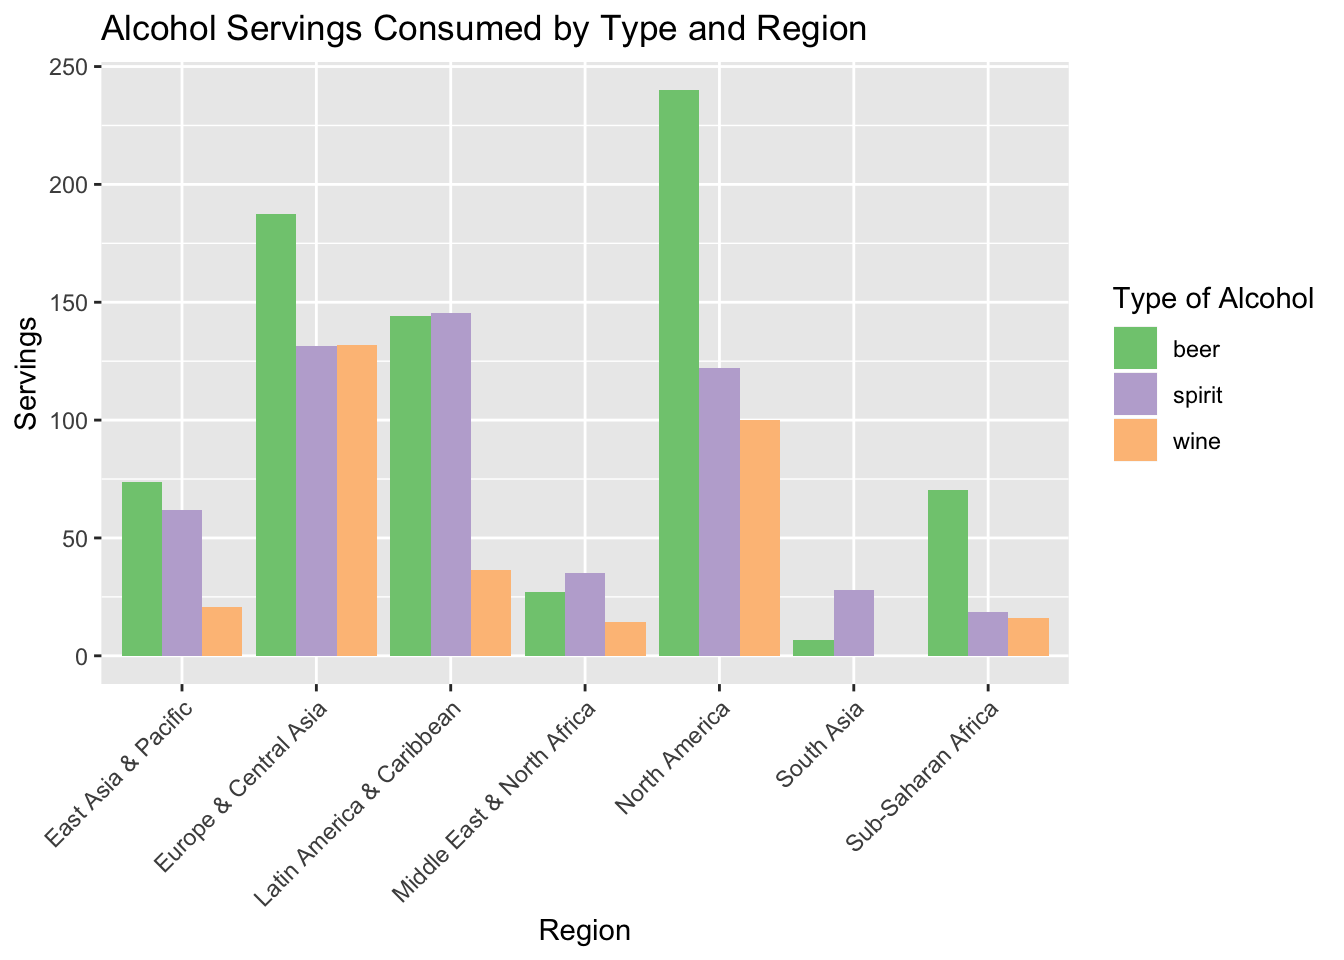
\includegraphics{project1_files/figure-latex/unnamed-chunk-11-1.pdf}

This graph shows the breakdown of the type of alcohol favored by members
of each region. Typically, if there is a type of alcohol that dominates
the others, it is beer as shown by North America, Europe \& Central
Asia, and Sub-Saharan Africa. Wine also tends to be consumed at the
lowest rate. North America, Europe \& Central Asia, and Latin America \&
Caribbean appear to be consuming the most servings. This is consistent
with the previous plot.

\subsection{Dimensionality Reduction}\label{dimensionality-reduction}

I'm going to run a PCA on this data. First, I'll set it all up by
scaling the numeric data and running princomp() to get some preliminary
info.

\begin{Shaded}
\begin{Highlighting}[]
\NormalTok{proj1num<-project1}\OperatorTok\KeywordTok{select_if}\NormalTok{(is.numeric)}\OperatorTok\NormalTok{scale}
\KeywordTok{rownames}\NormalTok{(proj1num)<-project1}\OperatorTok{$}\NormalTok{country}
\KeywordTok{head}\NormalTok{(proj1num)}
\end{Highlighting}
\end{Shaded}

\begin{verbatim}
##             total_litres_of_pure_alcohol    servings    GDP_pct total_servings
## Afghanistan                  -1.24252689 -0.85058477  0.7380062     -1.1282319
## Afghanistan                  -1.24252689 -0.85058477  0.7380062     -1.1282319
## Afghanistan                  -1.24252689 -0.85058477  0.7380062     -1.1282319
## Albania                       0.02653082  0.08725594 -0.5207003      0.1530105
## Albania                       0.02653082  0.54036999 -0.5207003      0.1530105
## Albania                       0.02653082 -0.28155782 -0.5207003      0.1530105
\end{verbatim}

\begin{Shaded}
\begin{Highlighting}[]
\NormalTok{proj1pca<-}\KeywordTok{princomp}\NormalTok{(proj1num)}
\KeywordTok{names}\NormalTok{(proj1pca)}
\end{Highlighting}
\end{Shaded}

\begin{verbatim}
## [1] "sdev"     "loadings" "center"   "scale"    "n.obs"    "scores"   "call"
\end{verbatim}

\begin{Shaded}
\begin{Highlighting}[]
\KeywordTok{summary}\NormalTok{(proj1pca, }\DataTypeTok{loadings=}\NormalTok{T)}
\end{Highlighting}
\end{Shaded}

\begin{verbatim}
## Importance of components:
##                           Comp.1    Comp.2     Comp.3     Comp.4
## Standard deviation     1.6722356 0.9005397 0.57255802 0.23812509
## Proportion of Variance 0.7005168 0.2031559 0.08212259 0.01420476
## Cumulative Proportion  0.7005168 0.9036727 0.98579524 1.00000000
## 
## Loadings:
##                              Comp.1 Comp.2 Comp.3 Comp.4
## total_litres_of_pure_alcohol  0.566  0.104  0.458  0.678
## servings                      0.507  0.274 -0.813       
## GDP_pct                       0.314 -0.941 -0.125       
## total_servings                0.569  0.171  0.338 -0.729
\end{verbatim}

It seems like component 1 explains a high proportion of variance.
Component 2 also explains a fair amount of variance. Let's make sure
these hunches are right by making a scree plot. From there I'll decide
how many components to use.

\begin{Shaded}
\begin{Highlighting}[]
\NormalTok{eigval<-proj1pca}\OperatorTok{$}\NormalTok{sdev}\OperatorTok{^}\DecValTok{2}
\NormalTok{varprop=}\KeywordTok{round}\NormalTok{(eigval}\OperatorTok{/}\KeywordTok{sum}\NormalTok{(eigval),}\DecValTok{2}\NormalTok{)}

\KeywordTok{ggplot}\NormalTok{()}\OperatorTok{+}\KeywordTok{geom_bar}\NormalTok{(}\KeywordTok{aes}\NormalTok{(}\DataTypeTok{y=}\NormalTok{varprop,}\DataTypeTok{x=}\DecValTok{1}\OperatorTok{:}\DecValTok{4}\NormalTok{),}\DataTypeTok{stat=}\StringTok{"identity"}\NormalTok{)}\OperatorTok{+}\KeywordTok{xlab}\NormalTok{(}\StringTok{""}\NormalTok{)}\OperatorTok{+}\KeywordTok{geom_path}\NormalTok{(}\KeywordTok{aes}\NormalTok{(}\DataTypeTok{y=}\NormalTok{varprop,}\DataTypeTok{x=}\DecValTok{1}\OperatorTok{:}\DecValTok{4}\NormalTok{))}\OperatorTok{+}
\StringTok{  }\KeywordTok{geom_text}\NormalTok{(}\KeywordTok{aes}\NormalTok{(}\DataTypeTok{x=}\DecValTok{1}\OperatorTok{:}\DecValTok{4}\NormalTok{,}\DataTypeTok{y=}\NormalTok{varprop,}\DataTypeTok{label=}\KeywordTok{round}\NormalTok{(varprop,}\DecValTok{2}\NormalTok{)),}\DataTypeTok{vjust=}\DecValTok{1}\NormalTok{,}\DataTypeTok{col=}\StringTok{"white"}\NormalTok{,}\DataTypeTok{size=}\DecValTok{5}\NormalTok{)}\OperatorTok{+}
\StringTok{  }\KeywordTok{scale_y_continuous}\NormalTok{(}\DataTypeTok{breaks=}\KeywordTok{seq}\NormalTok{(}\DecValTok{0}\NormalTok{,.}\DecValTok{6}\NormalTok{,.}\DecValTok{2}\NormalTok{),}\DataTypeTok{labels =}\NormalTok{ scales}\OperatorTok{::}\NormalTok{percent)}\OperatorTok{+}
\StringTok{  }\KeywordTok{scale_x_continuous}\NormalTok{(}\DataTypeTok{breaks=}\DecValTok{1}\OperatorTok{:}\DecValTok{10}\NormalTok{)}
\end{Highlighting}
\end{Shaded}

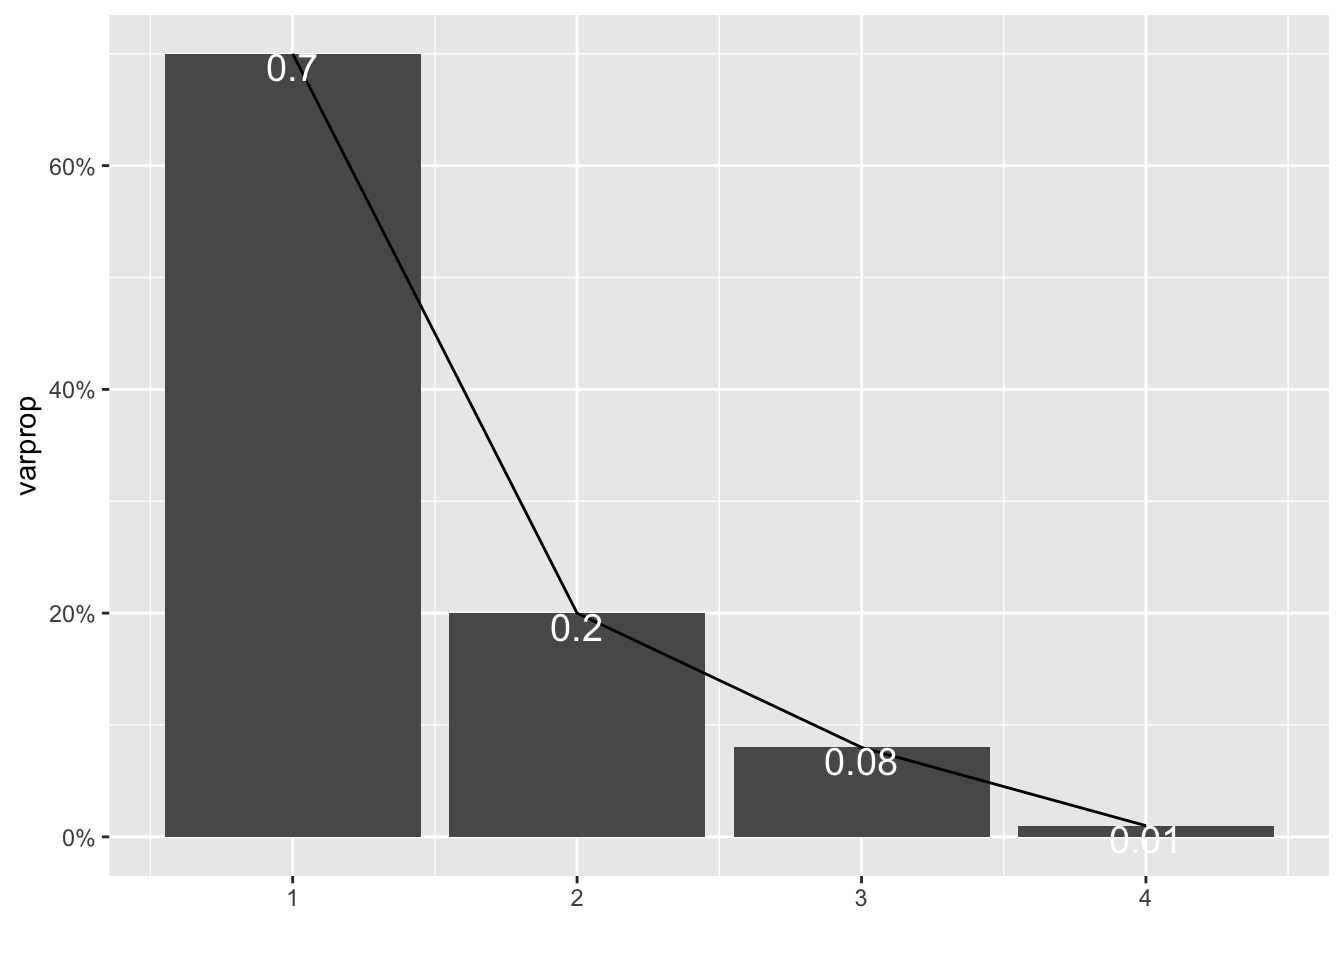
\includegraphics{project1_files/figure-latex/unnamed-chunk-13-1.pdf}

It seems that the elbow of this graph is at the second component. The
cumulative proportion of variance after this component is around 0.9 so
that seems like a good place to cut off. I'll include components 1 and 2
in my analysis. I'm going to pull up loadings again in order to
interpret the components.

\begin{Shaded}
\begin{Highlighting}[]
\NormalTok{proj1pca}\OperatorTok{$}\NormalTok{loadings}
\end{Highlighting}
\end{Shaded}

\begin{verbatim}
## 
## Loadings:
##                              Comp.1 Comp.2 Comp.3 Comp.4
## total_litres_of_pure_alcohol  0.566  0.104  0.458  0.678
## servings                      0.507  0.274 -0.813       
## GDP_pct                       0.314 -0.941 -0.125       
## total_servings                0.569  0.171  0.338 -0.729
## 
##                Comp.1 Comp.2 Comp.3 Comp.4
## SS loadings      1.00   1.00   1.00   1.00
## Proportion Var   0.25   0.25   0.25   0.25
## Cumulative Var   0.25   0.50   0.75   1.00
\end{verbatim}

For component 1, all of the variables have the same sign and similar
magnitude. Earlier, I found a slight correlation between percentage of
GDP spent on healthcare and alcohol consumption so it makes sense that
the first principle component would be dependent on strength of both of
these. For example, a country that spends little money on healthcare and
consumes a small amount of alcohol will have a high component 1 score.
On component 2, all of the variables share a sign except for percentage
of GDP spent on healthcare. It seems as though the trade-off between
healthcare spending and alcohol consumption controls this component. For
a score to have a higher magnitude on component 2, their healthcare
spending must be either very high or very low compared to their alcohol
consumption.

\begin{Shaded}
\begin{Highlighting}[]
\KeywordTok{ggplot}\NormalTok{()}\OperatorTok{+}\KeywordTok{geom_point}\NormalTok{(}\KeywordTok{aes}\NormalTok{(proj1pca}\OperatorTok{$}\NormalTok{scores[,}\DecValTok{1}\NormalTok{], proj1pca}\OperatorTok{$}\NormalTok{scores[,}\DecValTok{2}\NormalTok{]))}\OperatorTok{+}\KeywordTok{xlab}\NormalTok{(}\StringTok{"PC1"}\NormalTok{)}\OperatorTok{+}\KeywordTok{ylab}\NormalTok{(}\StringTok{"PC2"}\NormalTok{)}
\end{Highlighting}
\end{Shaded}

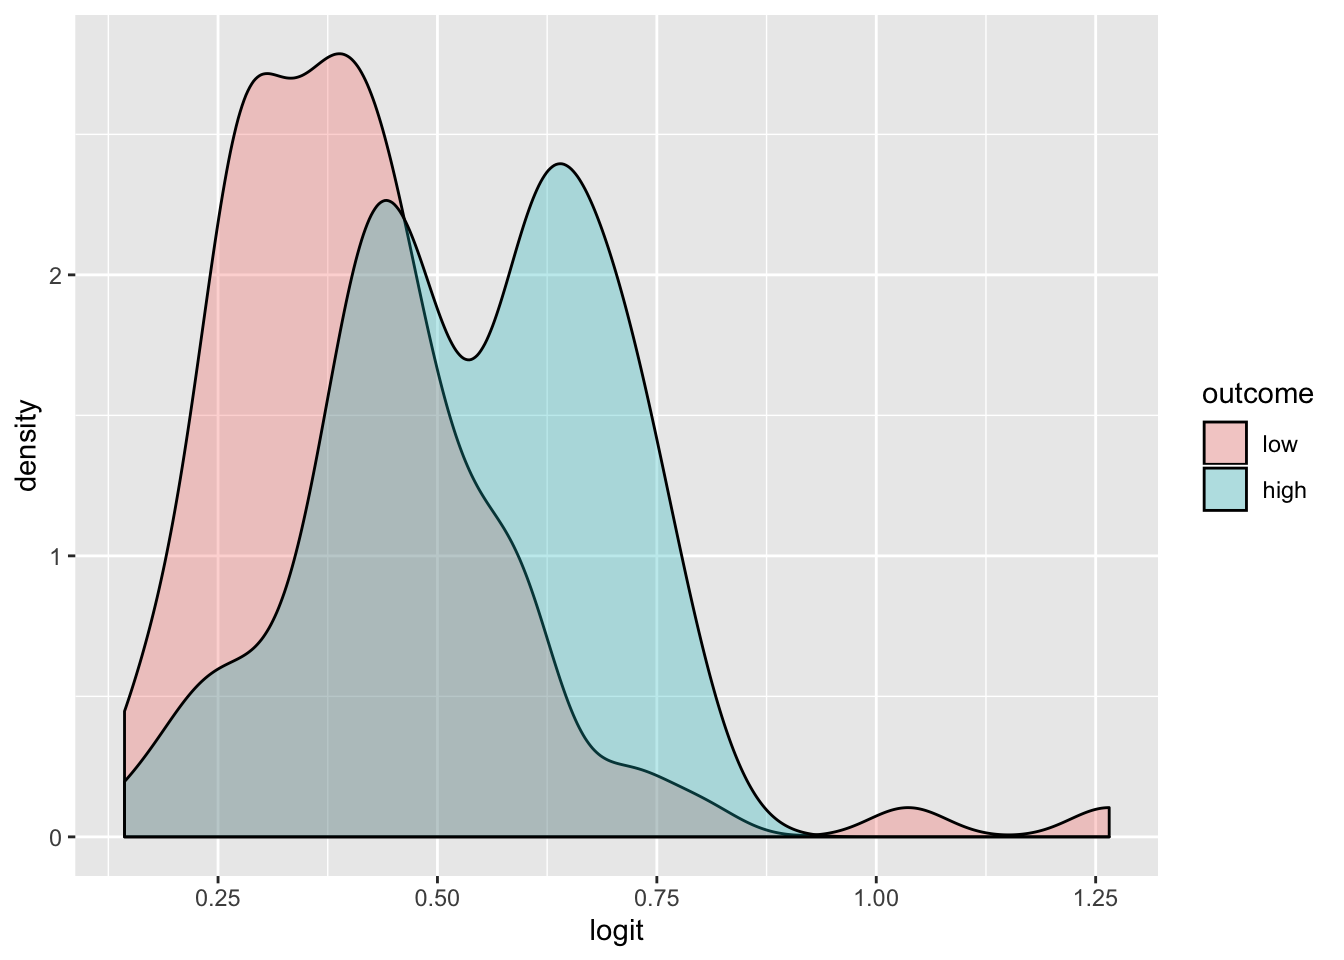
\includegraphics{project1_files/figure-latex/unnamed-chunk-15-1.pdf}

There are a few extreme points on PC2 - let's investigate!

\begin{Shaded}
\begin{Highlighting}[]
\NormalTok{Name<-project1}\OperatorTok{$}\NormalTok{country}
\NormalTok{proj1pca}\OperatorTok{$}\NormalTok{scores}\OperatorTok\NormalTok{as.data.frame}\OperatorTok\KeywordTok{cbind}\NormalTok{(Name,.)}\OperatorTok\KeywordTok{top_n}\NormalTok{(}\DecValTok{9}\NormalTok{,Comp.}\DecValTok{2}\NormalTok{)}\OperatorTok\KeywordTok{arrange}\NormalTok{(}\KeywordTok{desc}\NormalTok{(Comp.}\DecValTok{2}\NormalTok{))}
\end{Highlighting}
\end{Shaded}

\begin{verbatim}
##                 Name     Comp.1   Comp.2     Comp.3      Comp.4
## 1              Gabon  2.2749047 2.421178 -1.2034316  0.11155651
## 2  Equatorial Guinea  0.6317010 2.179787 -0.8353168  0.08646099
## 3         Kazakhstan  1.1314784 1.892061 -0.7910905  0.06572209
## 4  Equatorial Guinea -0.1222541 1.772069  0.3719743 -0.03741611
## 5             Angola  0.6785210 1.730717 -0.7492416  0.09619788
## 6 Russian Federation  3.1954530 1.717786 -0.6013129  0.03791555
## 7              Gabon  0.9434521 1.701165  0.9285932 -0.10720518
## 8            Grenada  4.0290554 1.690541 -1.5330735  0.12866362
## 9           Thailand  1.1469403 1.676382 -1.0084485  0.07979529
\end{verbatim}

\begin{Shaded}
\begin{Highlighting}[]
\NormalTok{project1}\OperatorTok\KeywordTok{filter}\NormalTok{(country}\OperatorTok{==}\StringTok{"Marshall Islands"}\OperatorTok{|}\NormalTok{country}\OperatorTok{==}\StringTok{"Tuvalu"}\NormalTok{)}
\end{Highlighting}
\end{Shaded}

\begin{verbatim}
## # A tibble: 6 x 7
##   country    total_litres_of_pu… type  servings GDP_pct region    total_servings
##   <chr>                    <dbl> <chr>    <int>   <dbl> <chr>              <int>
## 1 Marshall …                   0 beer         0    19.3 East Asi…              0
## 2 Marshall …                   0 spir…        0    19.3 East Asi…              0
## 3 Marshall …                   0 wine         0    19.3 East Asi…              0
## 4 Tuvalu                       1 beer         6    15.7 East Asi…             56
## 5 Tuvalu                       1 spir…       41    15.7 East Asi…             56
## 6 Tuvalu                       1 wine         9    15.7 East Asi…             56
\end{verbatim}

These points seem to refer to the Marshall Islands and Tuvalu. Upon
further investigation, it seems that these two have very low alcohol
consumption and high healthcare spending. This lines up with what I
noted as the parameters for component 2. I'll do this all again to see
the bottom scorers for PC1.

\begin{Shaded}
\begin{Highlighting}[]
\NormalTok{proj1pca}\OperatorTok{$}\NormalTok{scores}\OperatorTok\NormalTok{as.data.frame}\OperatorTok\KeywordTok{cbind}\NormalTok{(Name,.)}\OperatorTok\KeywordTok{top_n}\NormalTok{(}\DecValTok{5}\NormalTok{,}\DataTypeTok{wt=}\KeywordTok{desc}\NormalTok{(Comp.}\DecValTok{1}\NormalTok{))}\OperatorTok\KeywordTok{arrange}\NormalTok{(Comp.}\DecValTok{1}\NormalTok{)}
\end{Highlighting}
\end{Shaded}

\begin{verbatim}
##          Name    Comp.1    Comp.2      Comp.3      Comp.4
## 1 Timor-Leste -2.301783 1.1373655 -0.02291069 -0.03292566
## 2 Timor-Leste -2.301783 1.1373655 -0.02291069 -0.03292566
## 3 Timor-Leste -2.285742 1.1460403 -0.04859773 -0.03028997
## 4     Myanmar -2.259431 0.9914512 -0.03337902 -0.03885818
## 5     Myanmar -2.254084 0.9943428 -0.04194137 -0.03797962
\end{verbatim}

\begin{Shaded}
\begin{Highlighting}[]
\NormalTok{project1}\OperatorTok\KeywordTok{filter}\NormalTok{(country}\OperatorTok{==}\StringTok{"France"}\OperatorTok{|}\NormalTok{country}\OperatorTok{==}\StringTok{"Grenada"}\OperatorTok{|}\NormalTok{country}\OperatorTok{==}\StringTok{"Germany"}\OperatorTok{|}\NormalTok{country}\OperatorTok{==}\StringTok{"Andorra"}\OperatorTok{|}\NormalTok{country}\OperatorTok{==}\StringTok{"Belarus"}\NormalTok{)}
\end{Highlighting}
\end{Shaded}

\begin{verbatim}
## # A tibble: 15 x 7
##    country total_litres_of_pu… type   servings GDP_pct region     total_servings
##    <chr>                 <dbl> <chr>     <int>   <dbl> <chr>               <int>
##  1 Andorra                12.4 beer        245    9.45 Europe & …            695
##  2 Andorra                12.4 spirit      138    9.45 Europe & …            695
##  3 Andorra                12.4 wine        312    9.45 Europe & …            695
##  4 Belarus                14.4 beer        142    5.66 Europe & …            557
##  5 Belarus                14.4 spirit      373    5.66 Europe & …            557
##  6 Belarus                14.4 wine         42    5.66 Europe & …            557
##  7 France                 11.8 beer        127   11.2  Europe & …            648
##  8 France                 11.8 spirit      151   11.2  Europe & …            648
##  9 France                 11.8 wine        370   11.2  Europe & …            648
## 10 Germany                11.3 beer        346   11.0  Europe & …            638
## 11 Germany                11.3 spirit      117   11.0  Europe & …            638
## 12 Germany                11.3 wine        175   11.0  Europe & …            638
## 13 Grenada                11.9 beer        199    6.09 Latin Ame…            665
## 14 Grenada                11.9 spirit      438    6.09 Latin Ame…            665
## 15 Grenada                11.9 wine         28    6.09 Latin Ame…            665
\end{verbatim}

These countries have both high alcohol consumption and high healthcare
spending. Once again, this matches the parameters that I noted for
component 1.

Lets look at another graph to explain the roles the variables play in
both componenets.

\begin{Shaded}
\begin{Highlighting}[]
\NormalTok{proj1pca}\OperatorTok{$}\NormalTok{loadings[}\DecValTok{1}\OperatorTok{:}\DecValTok{4}\NormalTok{,}\DecValTok{1}\OperatorTok{:}\DecValTok{2}\NormalTok{]}\OperatorTok\NormalTok{as.data.frame}\OperatorTok\NormalTok{rownames_to_column}\OperatorTok
\KeywordTok{ggplot}\NormalTok{()}\OperatorTok{+}\KeywordTok{geom_hline}\NormalTok{(}\KeywordTok{aes}\NormalTok{(}\DataTypeTok{yintercept=}\DecValTok{0}\NormalTok{),}\DataTypeTok{lty=}\DecValTok{2}\NormalTok{)}\OperatorTok{+}
\StringTok{  }\KeywordTok{geom_vline}\NormalTok{(}\KeywordTok{aes}\NormalTok{(}\DataTypeTok{xintercept=}\DecValTok{0}\NormalTok{),}\DataTypeTok{lty=}\DecValTok{2}\NormalTok{)}\OperatorTok{+}\KeywordTok{ylab}\NormalTok{(}\StringTok{"PC2"}\NormalTok{)}\OperatorTok{+}\KeywordTok{xlab}\NormalTok{(}\StringTok{"PC1"}\NormalTok{)}\OperatorTok{+}
\StringTok{  }\KeywordTok{geom_segment}\NormalTok{(}\KeywordTok{aes}\NormalTok{(}\DataTypeTok{x=}\DecValTok{0}\NormalTok{,}\DataTypeTok{y=}\DecValTok{0}\NormalTok{,}\DataTypeTok{xend=}\NormalTok{Comp.}\DecValTok{1}\NormalTok{,}\DataTypeTok{yend=}\NormalTok{Comp.}\DecValTok{2}\NormalTok{),}\DataTypeTok{arrow=}\KeywordTok{arrow}\NormalTok{(),}\DataTypeTok{col=}\StringTok{"red"}\NormalTok{)}\OperatorTok{+}
\StringTok{  }\KeywordTok{geom_label}\NormalTok{(}\KeywordTok{aes}\NormalTok{(}\DataTypeTok{x=}\NormalTok{Comp.}\DecValTok{1}\OperatorTok{*}\FloatTok{1.1}\NormalTok{,}\DataTypeTok{y=}\NormalTok{Comp.}\DecValTok{2}\OperatorTok{*}\FloatTok{1.1}\NormalTok{,}\DataTypeTok{label=}\NormalTok{rowname))}\OperatorTok{+}\KeywordTok{expand_limits}\NormalTok{(}\DataTypeTok{x=}\OperatorTok{-}\FloatTok{0.8}\NormalTok{)}
\end{Highlighting}
\end{Shaded}

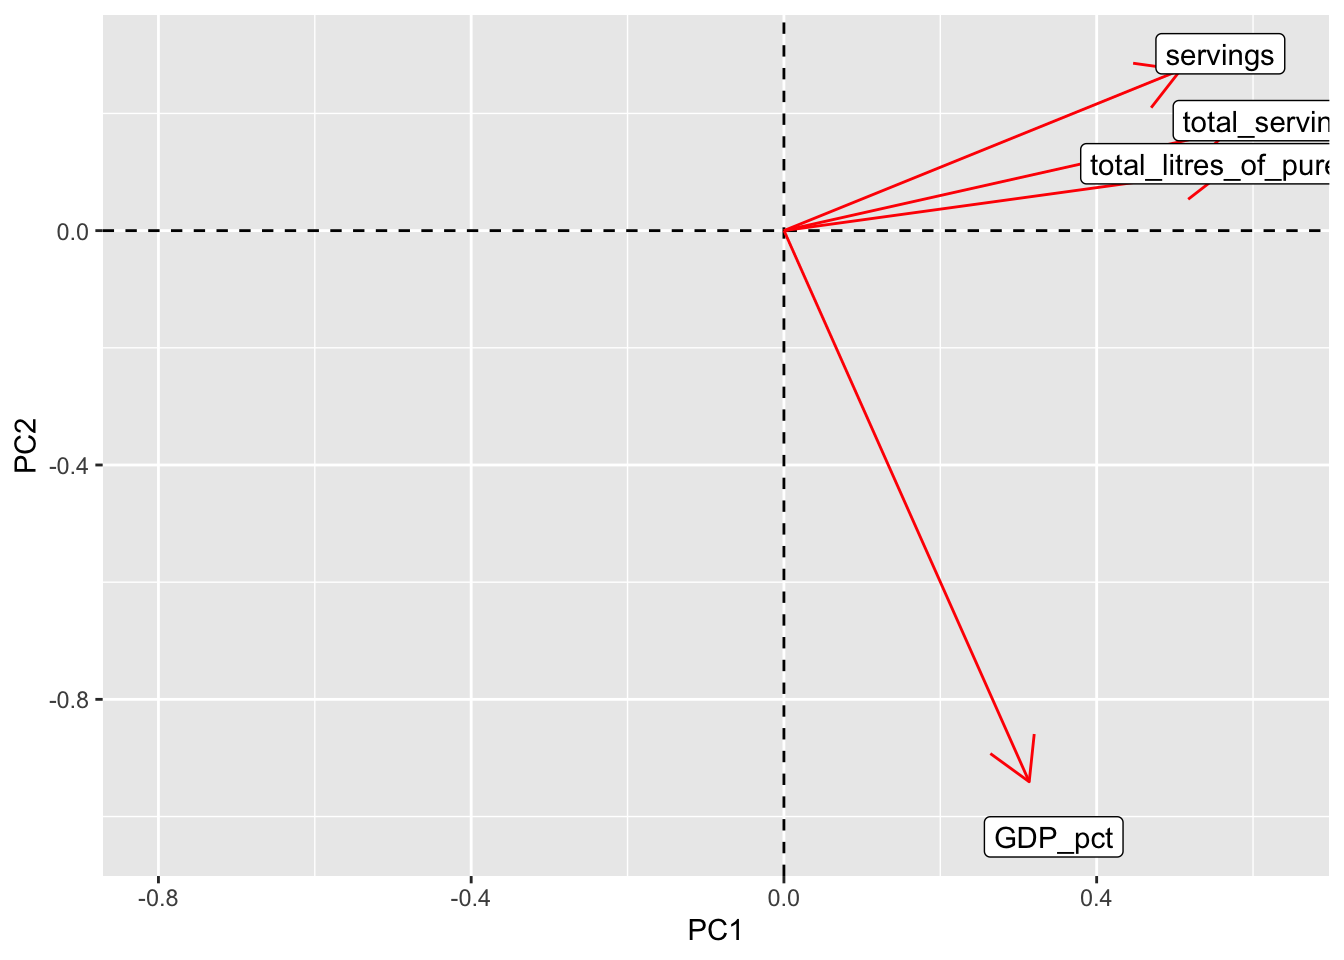
\includegraphics{project1_files/figure-latex/unnamed-chunk-18-1.pdf}

This graph simply confirms what I mentioned earlier. All of the
variables contribute to PC1 in the same way - when any of these values
is high, it contributes to a lower PC1 score. For PC2, the three alcohol
variables are in opposition to the GDP\_pct variable. When healthcare
spending is high and alcohol consumption is low, there is a high PC2
score.

\end{document}
